\documentclass[12pt, a4paper]{report}

% --- Encodage & langue ---
\usepackage[utf8]{inputenc}
\usepackage[T1]{fontenc}
\usepackage[french]{babel}
\usepackage{csquotes}

% --- Mise en page ---
\usepackage[top=2.5cm, bottom=2.5cm, left=3cm, right=2.5cm]{geometry}
\usepackage{setspace}
\onehalfspacing  % interligne 1.5

% --- Figures & tableaux ---
\usepackage{graphicx}
\graphicspath{{figures/}}   % mettre toutes les figures dans /figures
\usepackage{caption}
\usepackage{subcaption}
\usepackage{float}
\usepackage{tikz}
\usetikzlibrary{arrows.meta,calc}
\usepackage{booktabs}       % jolis tableaux

% --- Mathématiques ---
\usepackage{amsmath}
\usepackage{amssymb}

% --- Bibliographie ---
\usepackage[backend=biber, style=numeric, sorting=nyt]{biblatex}
\addbibresource{refs.bib}

% --- Hyperliens ---
\usepackage[colorlinks=true, linkcolor=black, citecolor=blue, urlcolor=blue]{hyperref}

% --- En-têtes & pieds de page ---
\usepackage{fancyhdr}
\setlength{\headheight}{15pt}
\pagestyle{fancy}
\fancyhf{}
\rhead{\leftmark}
\cfoot{\thepage}
\renewcommand{\headrulewidth}{0.4pt}

% --- Couleur (optionnel) ---
\usepackage{xcolor}

%  Page de garde
\title{
    {\Large Rapport de stage IR} \\[0.5em]
    {\huge \textbf{Génération de datasets synthétiques et tests Cross-dataset}} \\[1em]
    {\large Laboratoire CITI}
}
\author{
    Evan \textsc{JOASSON} \\[0.3em]
    \small Encadrant : Frédéric \textsc{Le MOUËL}
}
\date{1er juin -- 4 juillet 2026}


% ============================================================
\begin{document}
% ============================================================

% --- Page de titre ---
\maketitle
\thispagestyle{empty}
\newpage

% --- Remerciements ---
\chapter*{Remerciements}
\addcontentsline{toc}{chapter}{Remerciements}

Je tiens tout d’abord à remercier mon tuteur de stage, M. LE MOUËL, pour m'avoir accordé sa confiance et m'avoir donné l'opportunité d'effectuer ce stage de recherche au sein du laboratoire CITI de l'INSA, dont il est aussi le directeur. Je le remercie aussi pour son encadrement bienveillant, sa disponibilité, ainsi que pour les précieux conseils et l'accompagnement qu'il m'a apportés tout au long de ce projet.

Cette immersion au cœur de l'activité scientifique a été une expérience particulièrement enrichissante. Elle m'a permis d'appréhender concrètement la réalité du monde de la recherche, d'en comprendre la rigueur et les exigences méthodologiques, tout en développant un esprit critique face aux démarches expérimentales. Grâce à cette opportunité, j'ai pu non seulement affiner mes connaissances théoriques et pratiques, mais aussi découvert ce vaste domaine qu'est la recherche.

Mes remerciements s'étendent également à l'ensemble des membres du laboratoire pour leur accueil chaleureux,leur écoute, leur bienveillance et leur disponibilité au quotidien ont grandement contribué à faire de ce stage une excellente expérience, tant sur le plan humain que scientifique.

\newpage

% --- Résumé ---
\chapter*{Résumé}

La génération de datasets pour l'entraînement de systèmes de détection d'intrusions (IDS)
fondés sur l'apprentissage automatique constitue un défi majeur de la recherche en
cybersécurité. Ce stage a porté sur l'analyse de l'outil ID2T (\textit{Intrusion Detection
Dataset Toolkit}), qui permet d'injecter des attaques synthétiques dans du trafic réseau
bénin capturé au format \texttt{.pcap}, afin de produire des datasets étiquetés réalistes.
 
L'analyse structurelle de l'outil a mis en lumière son architecture modulaire et
déterministe, les features statistiques extraites du trafic source pour calibrer les
attaques injectées, ainsi qu'un bug silencieux du module Merger entraînant la perte du
trafic bénin lors du traitement de captures TON-IoT.
 
Afin d'évaluer empiriquement le réalisme du trafic d'attaque généré, un protocole de
benchmark cross-dataset a été mis en place. Un classifieur MLP est entraîné sur un
dataset généré par ID2T, puis évalué sur un dataset réel indépendant (CICIDS2017 ou
TON-IoT), et réciproquement. Les résultats montrent une forte asymétrie selon le
contexte réseau source, la généralisation est quasiment nulle sur un fond de réseau
classique (recall de 0,30\,\% en sens ID2T\,$\rightarrow$\,CICIDS2017), mais
sensiblement meilleure sur un fond de réseau IoT (recall de 78,29\,\% en sens
ID2T\,$\rightarrow$\,TON-IoT). Le trafic bénin, en revanche, s'est révélé fidèle au
trafic source dans tous les cas testés. Ces travaux confirment qu'ID2T est un outil
utile mais dont le réalisme des attaques générées doit être vérifié empiriquement
pour chaque contexte d'utilisation.

\newpage

% --- Table des matières ---
\tableofcontents
\newpage
 
% --- Liste des figures (optionnel) ---
\listoffigures
\listoftables
\newpage
 
 
% ============================================================
%  CORPS DU RAPPORT
% ============================================================
 
% --------------------------------------------------------
\chapter{Introduction}
% --------------------------------------------------------
 
\section{Contexte}
 
La détection d'intrusions dans les réseaux informatiques constitue un enjeu majeur de la cybersécurité moderne.
Les systèmes de détection d'intrusions (IDS, \textit{Intrusion Detection Systems}) visent à identifier
automatiquement des comportements malveillants au sein du trafic réseau.
L'essor des approches par apprentissage profond (\textit{Deep Learning}) a ouvert de nouvelles perspectives pour
ces systèmes, permettant de dépasser les limites des méthodes à base de règles ou de signatures statiques.
 
Cependant, l'entraînement de tels modèles requiert des jeux de données (\textit{datasets}) de trafic réseau
étiquetés, c'est-à-dire contenant à la fois du trafic bénin et des exemples d'attaques annotés.
La constitution de ces datasets représente un défi, car, capturer du trafic malveillant réel soulève des
contraintes éthiques et opérationnelles importantes, et les datasets publics disponibles peinent souvent
à refléter la diversité des environnements réseau réels.
 
\section{Problématique}
 
Une approche prometteuse pour contourner ces difficultés consiste à \textit{injecter} synthétiquement des
attaques dans du trafic réseau bénin existant, afin de produire des datasets réalistes et contrôlés.
L'outil \textbf{ID2T} (\textit{Intrusion Detection Dataset Toolkit}) a été développé dans cette optique, il permet d'injecter différents types d'attaques dans un fichier de capture de trafic réseau au format \texttt{.pcap}, tout en cherchant à préserver la cohérence statistique du trafic résultant.
 
Toutefois, la qualité et la validité des datasets générés dépendent directement de la pertinence des
caractéristiques (\textit{features}) utilisées lors de l'injection, ainsi que de la capacité de l'outil à
s'adapter à des environnements réseau variés.
En particulier, des réseaux de type IoT (\textit{Internet of Things}) présentent des propriétés protocolaires
spécifiques, telles que des valeurs de TTL (\textit{Time To Live}) différentes de celles d'un réseau
informatique classique, qui peuvent remettre en question la cohérence des attaques injectées.
 
\section{Objectifs du stage}
 
L'objectif principal de ce stage est de mener une \textbf{analyse approfondie d'ID2T}.
Il s'agit d'examiner les features exploitées par l'outil pour modéliser et générer le trafic d'attaque,
d'évaluer son adaptabilité à différents types de réseaux, et d'étudier la cohérence des attaques injectées
en fonction des protocoles présents dans le trafic bénin source, avec une attention particulière portée
aux environnements IoT.
 
Dans un second temps, une \textbf{amélioration de l'outil} était envisagée, portant sur la prise en charge
de plusieurs fichiers \texttt{.pcap} en entrée afin de permettre la génération de datasets mixtes.
Par manque de temps, cet axe n'a pas pu être abordé durant le stage, il constitue néanmoins une perspective directe des travaux réalisés, discutée en conclusion.
 
\section{Plan du rapport}
 
La suite de ce rapport est organisée comme suit.
Le chapitre~\ref{chap:etat_art} présente l'état de l'art sur les IDS, les datasets de trafic réseau pour
l'apprentissage automatique, et introduit l'outil ID2T.
Le chapitre~\ref{chap:analyse} détaille l'analyse menée sur ID2T~: fonctionnement interne, features
utilisées, adaptabilité et cohérence des attaques selon les protocoles.
Le chapitre~\ref{chap:mlp} décrit le protocole d'évaluation cross-dataset mis en place pour mesurer le réalisme du trafic généré par ID2T à l'aide d'un MLP, et en présente les résultats.
Le chapitre~\ref{chap:discussion} discute les résultats obtenus et les limites du travail réalisé.
Enfin, le chapitre~\ref{chap:conclusion} conclut ce rapport et présente les perspectives envisageables
pour la suite de ces travaux, notamment l'amélioration de l'outil.
 
 
% --------------------------------------------------------
\chapter{État de l'art}
\label{chap:etat_art}
 
\section{Détection d'intrusions réseau et apprentissage automatique}
 
Les systèmes de détection d'intrusions réseau (NIDS, \textit{Network Intrusion Detection Systems})
ont pour objectif d'identifier, au sein du trafic réseau, des comportements anormaux ou malveillants.
Deux grandes familles coexistent dans la littérature.
Les approches \textit{à base de signatures} détectent les attaques par correspondance avec un catalogue
de patterns connus~: elles sont efficaces contre les menaces répertoriées mais échouent dès qu'un
attaquant modifie légèrement son approche.
Les approches \textit{par détection d'anomalies} modélisent au contraire le trafic normal et signalent
tout écart significatif, offrant une capacité de généralisation absente des systèmes à
signatures~\cite{sharafaldin2018}.
 
L'essor de l'apprentissage automatique (\textit{machine learning}, ML) a substantiellement amélioré
les performances de la détection d'anomalies~\cite{survey2026}. Parmi les architectures employées,
le perceptron multicouche (\textit{Multilayer Perceptron}, MLP) constitue la référence la plus
directe, opérant sur des vecteurs de features extraites des flux réseau, il offre un bon équilibre
entre simplicité d'implémentation et capacité de classification, ce qui en fait un choix naturel pour
évaluer la qualité d'un dataset et servir de baseline reproductible. La contrepartie commune à toutes
ces approches est leur exigence en données. Entraîner un tel modèle requiert de larges volumes de
trafic réseau correctement étiqueté, ce qui déplace le problème de la détection vers celui de la
constitution de datasets appropriés.
 
\section{Datasets de trafic réseau pour les NIDS}
 
\subsection{Principaux benchmarks et leurs limitations}
 
La recherche sur les NIDS repose depuis plusieurs décennies sur un petit nombre de datasets de
référence. Ring et al.~\cite{ring2019} en ont recensé et analysé les propriétés dans une revue
couvrant plus de trente jeux de données. Le tableau~\ref{tab:datasets} présente les quatre benchmarks
les plus fréquemment rencontrés dans la littérature.
 
\begin{table}[H]
\centering
\caption{Principaux datasets de référence pour les NIDS et leurs limitations connues~\cite{survey2025}.}
\label{tab:datasets}
\small
\begin{tabular}{lcccp{5.7cm}}
\toprule
\textbf{Dataset} & \textbf{Année} & \textbf{Chiffré} & \textbf{Étiqueté} & \textbf{Problèmes principaux} \\
\midrule
NSL-KDD    & 2009 & Non     & Oui & Attaques obsolètes, artefacts statistiques, réseau militaire simulé \\
UNSW-NB15  & 2015 & Non     & Oui & Déséquilibre de classes, chevauchement, conditions testbed \\
CICIDS2017 & 2017 & Non     & Oui & Erreurs d'étiquetage (CICFlowMeter), trafic bénin peu réaliste \\
TON-IoT    & 2020 & Partiel & Oui & Déséquilibre sévère (96\,\% d'attaques), mauvaise généralisation \\
\bottomrule
\end{tabular}
\end{table}
 
\textbf{NSL-KDD} corrige les redondances de son prédécesseur KDD99, mais hérite de ses conditions
réseau datant d'un testbed militaire de 1998. Des artefacts structurels, comme des valeurs de TTL et adresses IP systématiquement différentes entre trafic bénin et trafic d'attaque, permettent à des classifieurs naïfs d'atteindre une précision quasi-parfaite sans apprendre le moindre comportement réseau
significatif~\cite{survey2025}.
 
\textbf{UNSW-NB15}~\cite{moustafa2015} introduit une gamme plus large de types d'attaques modernes,
mais souffre d'un déséquilibre de classes prononcé et d'un chevauchement entre les distributions
bénignes et malveillantes, rendant toute frontière de décision difficile à apprendre~\cite{zoghi2024}.
 
\textbf{CICIDS2017}~\cite{sharafaldin2018} est devenu le benchmark de facto du domaine, totalisant
plus de 4\,200 citations à fin 2024~\cite{concap2026}. Engelen et al.~\cite{engelen2021} ont
cependant mis en évidence des erreurs d'étiquetage systématiques dues à une implémentation
défectueuse de CICFlowMeter, comme des terminaison incorrecte des flux TCP, ignorance des paquets RST,
conduisant à des échantillons mal étiquetés qui biaisent silencieusement tout classifieur entraîné.
 
\textbf{TON-IoT}~\cite{alsaedi2020} cible la sécurité des réseaux IoT et couvre neuf catégories
d'attaques. Son principal défaut est un déséquilibre de classes extrême, les attaques représentent
96,44\,\% des enregistrements~\cite{dinh2026}, ce qui pousse les modèles à classifier presque tout
trafic comme malveillant.
 
\subsection{Défauts de conception récurrents}
 
Au-delà des problèmes propres à chaque dataset, Flood et al.~\cite{flood2024} ont identifié
six défauts de conception récurrents dans les benchmarks NIDS, dans un article distingué
\textit{Best Paper} à IEEE EuroS\&P 2024, diversité de features limitée, forte interdépendance
entre features, vérité terrain ambiguë, effondrement des distributions de trafic, diversité
artificiellement générée et imprécisions d'étiquetage.
 
Le \textbf{déséquilibre de classes} est parmi les plus présents. Dans les réseaux réels, les
attaques constituent des événements rares, un classifieur qui étiquette tout flux comme bénin
atteindrait une précision supérieure à 99\,\% sur la plupart des captures, sans détecter la
moindre intrusion.
 
La \textbf{non-représentativité} du trafic est une problématique tout aussi sérieuse. Layeghy
et Portmann~\cite{layeghy2022} ont comparé les propriétés statistiques du trafic bénin de
CICIDS2017, UNSW-NB15 et TON-IoT à des captures réseau réelles et constaté des divergences
substantielles sur les distributions de taille de paquets, les temps inter-arrivée et les ratios
de protocoles. Leur conclusion est directe~: de bonnes performances sur les benchmarks synthétiques
ne garantissent pas l'efficacité en déploiement réel.
 
Enfin, des \textbf{fuites de features} (\textit{feature leakage}) ont été documentées.
Certaines caractéristiques comme les adresses IP ou ports spécifiques aux outils d'attaque,
horodatages séparant parfaitement les journées d'attaque des journées bénignes. Ces caractéristiques constituent des raccourcis non intentionnels qui gonflent artificiellement les métriques tout en rendant
le modèle inutilisable sur tout autre réseau~\cite{flood2024}.
 
L'ensemble de ces constats dresse un tableau cohérent, les datasets disponibles sont soit trop
anciens, soit mal étiquetés, soit statistiquement non représentatifs, soit aveugles au trafic
chiffré~\cite{hikari2021}. Générer de nouveaux datasets, correctement étiquetés et réalistes,
reste un défi ouvert.
 
\section{Génération de trafic réseau}
 
\subsection{Taxonomie des approches}
 
Adeleke et al.~\cite{adeleke2022} ont proposé une taxonomie des outils de génération de trafic
réseau en quatre familles, chacune présentant des compromis distincts entre réalisme,
flexibilité et reproductibilité (tableau~\ref{tab:taxonomy} et figure~\ref{fig:taxonomy}).
 
\begin{table}[H]
\centering
\caption{Comparaison des quatre familles d'outils de génération de trafic réseau.}
\label{tab:taxonomy}
\small
\begin{tabular}{p{3cm} p{3.7cm} p{1.5cm} p{1.6cm} p{3.5cm}}
\toprule
\textbf{Famille} & \textbf{Outils} & \textbf{Réalisme} & \textbf{Flexibilité} & \textbf{Limitation principale} \\
\midrule
Replay de trafic & Tcpreplay & Élevé & Faible & Figé dans le temps, sans état \\
Génération de paquets & Scapy, D-ITG, iPerf, TRex & Faible & Élevée & Aucun réalisme comportemental \\
Synthétique et injection & ID2T, HIKARI-2021, GAN & Élevé & Moyen & Dépend d'une capture réelle existante \\
Environnements conteneurisés & DetGen, ConCap & Élevé & Élevée & Infrastructure à déployer (Docker, Kubernetes) \\
\bottomrule
\end{tabular}
\end{table}
 
\begin{figure*}[!t]
\centering
\resizebox{\textwidth}{!}{%
\begin{tikzpicture}[
  every node/.style={draw, rounded corners, align=center, font=\footnotesize, inner sep=6pt},
  root/.style={fill=gray!15, minimum width=6.5cm, minimum height=0.8cm, font=\small\bfseries},
  family/.style={fill=blue!8, text width=3.6cm, minimum height=2.1cm},
  >=Stealth
]
\node[root] (root) at (0,0) {Outils de génération de trafic réseau};

\node[family] (replay)    at (-9.3,-3.0) {\textbf{Replay de trafic}\\[3pt] Tcpreplay\\[3pt] \textit{Haute fidélité, figé dans le temps}};
\node[family] (crafting)  at (-3.1,-3.0) {\textbf{Génération de paquets}\\[3pt] Scapy, D-ITG, iPerf, TRex\\[3pt] \textit{Haut débit, faible réalisme comportemental}};
\node[family] (synthetic) at (3.1,-3.0)  {\textbf{Synthétique et injection}\\[3pt] ID2T, HIKARI-2021, GAN\\[3pt] \textit{Statistiquement réaliste ; GANs difficiles à entraîner}};
\node[family] (container) at (9.3,-3.0)  {\textbf{Environnements conteneurisés}\\[3pt] DetGen, ConCap\\[3pt] \textit{Reproductible, scalable, étiqueté automatiquement}};

\draw (root.south) -- (0,-1.0);
\draw (-9.3,-1.0) -- (9.3,-1.0);
\draw[->] (-9.3,-1.0) -- (replay.north);
\draw[->] (-3.1,-1.0) -- (crafting.north);
\draw[->] (3.1,-1.0)  -- (synthetic.north);
\draw[->] (9.3,-1.0)  -- (container.north);
\end{tikzpicture}%
}
\caption{Taxonomie des familles d'outils de génération de trafic réseau~\cite{adeleke2022}.}
\label{fig:taxonomy}
\end{figure*}
 
\subsection{Replay de trafic}
 
Les outils de replay, tels que Tcpreplay, relisent un fichier PCAP préenregistré et retransmettent
ses paquets sur une interface réseau active. Cette approche préserve les propriétés statistiques
d'une capture réelle, mais n'offre aucune flexibilité, le trafic est figé dans le temps,
reflète un environnement réseau particulier, et ne permet d'introduire aucun nouveau scénario
d'attaque. De surcroît, la plupart de ces outils sont sans état et ne peuvent pas reconstruire
la nature bidirectionnelle d'une connexion réseau~\cite{survey2025}.
 
\subsection{Génération de paquets et tests de performance}
 
Cette famille regroupe des outils orientés vers la construction arbitraire de paquets ou les
tests de montée en charge~: Scapy, D-ITG, iPerf, TRex ou Ostinato. Une comparaison quantitative
de trois d'entre eux~\cite{koay2021} montre que, si leurs performances en débit sont élevées,
le trafic produit manque de réalisme. Les charges utiles sont absentes ou générées
aléatoirement, et les flux finaux ne ressemblent pas à du trafic applicatif réel.
 
\subsection{Approches synthétiques et par injection}
 
Les approches synthétiques et par injection constituent le compromis le plus adapté à la
génération de datasets pour IDS~\cite{adeleke2022}. Au lieu de créer du trafic en partant de zéro,
elles injectent des attaques synthétiques dans une capture bénigne existante, en veillant à
ce que le trafic injecté reste statistiquement cohérent avec le trafic environnant.
 
Garcia Cordero et al.~\cite{id2t2021} ont développé \textbf{ID2T} (\textit{Intrusion
Detection Dataset Toolkit}) selon ce principe~: à partir d'un fichier PCAP bénin, l'outil
en extrait une empreinte statistique (distribution de TTL, taille des paquets, entropie des
adresses IP, etc.) et contraint les paquets d'attaque injectés à reproduire ces propriétés,
de sorte que le trafic synthétique reste statistiquement indiscernable de trafic ayant
traversé le même réseau réel.
Dans une approche complémentaire, Ferriyan et al.~\cite{hikari2021} ont produit le dataset
HIKARI-2021 en ciblant spécifiquement le trafic d'attaque chiffré (TLS/HTTPS), comblant une
lacune ignorée par la majorité des outils existants.
Des approches génératives fondées sur des réseaux antagonistes génératifs
(GAN)~\cite{ring2019gan} ont également été proposées, mais restent difficiles à entraîner
et peinent à capturer les dépendances temporelles et les contraintes protocolaires
caractéristiques du trafic réseau réel.
 
\subsection{Environnements conteneurisés}
 
La quatrième famille exploite la conteneurisation pour générer du trafic étiqueté de manière
reproductible. DetGen~\cite{detgen2021} fut parmi les premiers outils de ce type, s'appuyant
sur Docker pour orchestrer des hôtes attaquants et victimes.
ConCap (\textit{Container Capture})~\cite{concap2026} pousse cette logique plus loin. Basé
sur Kubernetes, il supporte l'exécution concurrente de scénarios d'attaque multiples, un contrôle
fin des conditions réseau (bande passante, latence, perte de paquets) et l'extraction automatique
de NetFlows étiquetés. Sa validation empirique démontre que des classifieurs entraînés dans un
environnement conteneurisé généralisent efficacement à un réseau physique équivalent~\cite{concap2026}.
 
\section{Synthèse~: positionnement d'ID2T}
 
Parmi les approches les plus matures, ID2T et ConCap incarnent deux philosophies fondamentalement
opposées face au même objectif.
 
ID2T hérite de l'empreinte topologique d'un réseau réel via sa capture bénigne source~: les
propriétés infrastructurelles (distribution de TTL, comportements de routage, etc..) sont présentes
de facto dans le trafic de fond, sans qu'il soit nécessaire de les simuler. ConCap quant à lui génère
en revanche l'intégralité de son trafic dans un réseau de pods Kubernetes plat, sans NAT ni
routage intermédiaire, et ne laisse au chercheur le contrôle que des caractéristiques du
canal point-à-point.
 
ID2T préserve ainsi le réalisme topologique au prix d'une dépendance à une capture réelle et aux préoccupations de confidentialité associées. ConCap s'affranchit de cette dépendance en sacrifiant ce réalisme topologique. Ni l'un ni l'autre ne traitent explicitement le déséquilibre de classes ou les fuites de features, et la validation de ConCap en matière de représentativité reste limitée à un sous-ensemble restreint d'activités réseau~\cite{concap2026}.
 
\begin{figure}[H]
\centering
\resizebox{\linewidth}{!}{%
\begin{tikzpicture}[
  every node/.style={draw, rounded corners, align=center, font=\footnotesize, inner sep=6pt},
  header/.style={fill=gray!15, minimum width=6.5cm, font=\small\bfseries},
  procbox/.style={fill=blue!8, text width=6.5cm, minimum height=1.3cm},
  tradeoff/.style={fill=orange!12, text width=6.5cm, minimum height=1.7cm, font=\footnotesize\itshape},
  >=Stealth
]
\node[header]   (id2t-h) at (-4.5,0)    {ID2T - Synthétique et injection};
\node[procbox]  (id2t-1) at (-4.5,-2.0) {Capture bénigne réelle en entrée (PCAP)};
\node[procbox]  (id2t-2) at (-4.5,-4.0) {Extraction de l'empreinte statistique~: TTL, taille des paquets, entropie IP\ldots};
\node[procbox]  (id2t-3) at (-4.5,-6.0) {Injection des attaques contraintes à reproduire ces statistiques};
\node[tradeoff] (id2t-t) at (-4.5,-8.3) {Compromis~: dépend toujours d'une capture réelle + la confidentialité n'est que partiellement préservée};
 
\draw[->] (id2t-h) -- (id2t-1);
\draw[->] (id2t-1) -- (id2t-2);
\draw[->] (id2t-2) -- (id2t-3);
\draw[->] (id2t-3) -- (id2t-t);
 
\node[header]   (cc-h) at (4.5,0)    {ConCap - Environnement conteneurisé};
\node[procbox]  (cc-1) at (4.5,-2.0) {Déploiement attaquant/cible en pods Kubernetes isolés};
\node[procbox]  (cc-2) at (4.5,-4.0) {Réseau de pods plat~: pas de NAT, pas de routeurs ni pare-feux simulés};
\node[procbox]  (cc-3) at (4.5,-6.0) {Contrôle limité aux caractéristiques du canal~: bande passante, latence, pertes};
\node[tradeoff] (cc-t) at (4.5,-8.3) {Compromis~: absence de topologie réelle - routing asymétrique et inspection pare-feu non modélisables};
 
\draw[->] (cc-h) -- (cc-1);
\draw[->] (cc-1) -- (cc-2);
\draw[->] (cc-2) -- (cc-3);
\draw[->] (cc-3) -- (cc-t);
\end{tikzpicture}%
}
\caption{ID2T et ConCap~: deux philosophies opposées pour la génération de trafic étiqueté~\cite{id2t2021, concap2026}.}
\label{fig:id2t_vs_concap}
\end{figure}
 
C'est dans ce contexte qu'ID2T constitue l'objet central de ce stage. Son approche par
injection dans une capture réelle en fait un outil aux possibilités étendues, mais également
porteur de questions ouvertes sur la qualité des features utilisées et sur la cohérence des
attaques injectées selon les protocoles présents dans le trafic source, notamment dans
des environnements spécifiques tels que les réseaux IoT.
 
 
% --------------------------------------------------------
\chapter{Analyse d'ID2T}
\label{chap:analyse}
% --------------------------------------------------------
 
\section{Architecture et fonctionnement général}

ID2T est une application modulaire déterministe, pour une même entrée et les mêmes paramètres, elle produit toujours le même résultat. Elle ne repose sur aucun apprentissage automatique. Son réalisme repose entièrement sur des statistiques extraites du trafic bénin source.

L'outil prend en entrée un fichier \texttt{.pcap} de trafic bénin et un
ensemble de paramètres définis par l'utilisateur, et produit trois
artefacts~: un \texttt{.pcap} de sortie contenant le trafic fusionné
(bénin + attaques injectées), un fichier de labels au format XML
horodatant précisément chaque attaque, et un rapport TIDED.
L'architecture interne, illustrée en figure~\ref{fig:id2t_archi},
s'articule autour de sept modules.

\begin{figure}[H]
    \centering
    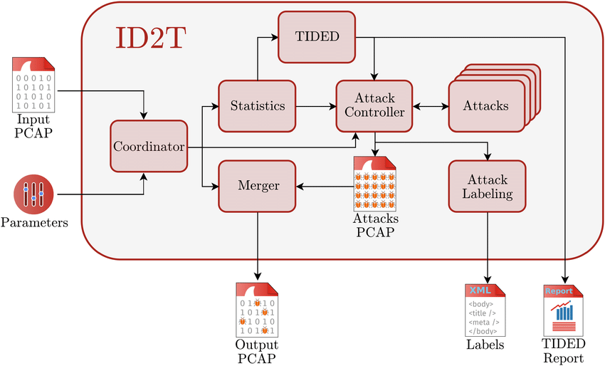
\includegraphics[width=0.85\linewidth]{id2t_architecture.png}
    \caption{Architecture d'ID2T et ses sept modules~\cite{id2t2021}.}
    \label{fig:id2t_archi}
\end{figure}
\newpage

Le \textbf{Coordinator} constitue le point d'entrée de l'outil, il
analyse la commande CLI, valide les paramètres fournis par l'utilisateur
et orchestre l'enchaînement des autres modules.

Le module \textbf{Statistics} parcourt l'intégralité du \texttt{.pcap}
source et consigne les propriétés statistiques du trafic dans une base
SQLite mise en cache, réutilisée lors de lancements ultérieurs sur le
même fichier. C'est le module central pour le réalisme du trafic injecté, son rôle est détaillé en section~\ref{sec:features}.

\textbf{TIDED} (\textit{Traffic-based Intrusion Detection Evasion and
Dataset generation}) analyse le trafic pour évaluer la détectabilité des
attaques générées et produit le rapport éponyme.

L'\textbf{Attack Controller} coordonne la génération du trafic malveillant,
il instancie le script d'attaque approprié, l'alimente avec les
statistiques extraites par le module Statistics, et produit un
\texttt{.pcap} intermédiaire contenant uniquement les paquets d'attaque
(\textit{Attacks PCAP}).

Le sous-système \textbf{Attacks} regroupe l'ensemble des implémentations
d'attaques disponibles, chacune sous forme de script Python indépendant~:
port scan, DDoS, EternalBlue, etc. Cette architecture facilite l'ajout
de nouveaux types d'attaques sans modifier le cœur de l'outil.

\textbf{Attack Labeling} génère le fichier XML de labels en annotant
précisément les intervalles temporels correspondant aux attaques injectées.

Enfin, le \textbf{Merger} fusionne le \texttt{.pcap} de trafic bénin
source et le \texttt{.pcap} d'attaques en un unique fichier de sortie,
en respectant l'ordre chronologique des paquets.



 
\section{Features utilisées pour la génération de trafic}
\label{sec:features}

Le module Statistics est au cœur du réalisme statistique d'ID2T. Il
extrait du \texttt{.pcap} source un ensemble de caractéristiques qui
servent à contraindre les paquets générés par l'Attack Controller,
afin qu'ils soient statistiquement cohérents avec le trafic bénin
environnant. Le tableau~\ref{tab:features} liste les principales
features extraites et leur usage lors de l'injection.

\begin{table}[H]
\centering
\caption{Features extraites par le module Statistics et leur rôle dans
la génération du trafic d'attaque.}
\label{tab:features}
\small
\begin{tabular}{p{5.5cm} p{8.5cm}}
\toprule
\textbf{Feature extraite} & \textbf{Usage lors de l'injection} \\
\midrule
Distribution des TTL par hôte     & Calibrer les valeurs de TTL des paquets d'attaque \\
IPs source/destination actives    & Sélectionner des adresses IP vraisemblables \\
Ports ouverts par sous-réseau     & Cibler des ports cohérents avec le réseau \\
Taille moyenne des paquets        & Dimensionner les payloads selon le protocole \\
Packet rate (paquets/s)           & Contrôler le débit et le timing de l'injection \\
Fenêtres TCP et checksums         & Générer des en-têtes TCP valides et cohérents \\
Entropie des adresses IP          & Évaluer la diversité des hôtes du réseau \\
\bottomrule
\end{tabular}
\end{table}

Toutes ces valeurs sont stockées dans une base SQLite locale, mise en
cache après le premier traitement d'un fichier. Un second lancement
sur le même \texttt{.pcap} recharge les statistiques sans recalcul,
réduisant significativement le temps d'exécution.
Il est important de noter qu'ID2T ne procède à aucun apprentissage,
le processus est entièrement déterministe et reproductible.
 
 
 
 
\section{Adaptabilité à différents types de réseaux}

Afin d'évaluer la capacité d'ID2T à traiter des environnements réseau
variés, l'attaque PortScan a été injectée dans deux types de captures
bénignes~: un fichier issu de CICIDS2017, représentatif d'un réseau
informatique classique, et un fichier issu de TON-IoT~\cite{alsaedi2020},
représentatif d'un environnement simulant des équipements IoT et IIoT.
Il est important de noter que TON-IoT repose sur des protocoles réseau
standards (TCP, UDP, ICMP) et non sur des protocoles applicatifs IoT
spécifiques tels que MQTT ou CoAP~\cite{dinh2026}.

Sur le trafic \textbf{CICIDS2017}, l'outil se comporte comme attendu,
le \texttt{.pcap} de sortie contient le trafic bénin source augmenté
des paquets d'attaque injectés, et le fichier de labels XML est généré
correctement.

Sur le trafic \textbf{TON-IoT}, un comportement anormal a été constaté,
le \texttt{.pcap} produit en sortie ne contient plus que les paquets
d'attaque, le trafic bénin source a entièrement disparu du fichier
de sortie. L'outil termine son exécution sans erreur apparente, et aucun message
d'avertissement n'est émis pour signaler la perte du trafic de fond.

La cause exacte de ce comportement n'a pas pu être identifiée faute de temps pour analyser les logs internes ou
le code source. Une piste probable concerne le module \textbf{Merger},il a pu être
confronté à certaines caractéristiques des paquets bénins de TON-IoT, ce trafic bénin est synthétique et non issu d'une capture réseau réelle, et le module pourrait échouer silencieusement à fusionner les deux flux.




\section{Cohérence des attaques selon les protocoles}
\label{sec:coherence}

Concernant la \textbf{cohérence des valeurs de TTL}, aucune anomalie
n'a été observée sur les captures testées. Ce résultat s'explique
directement par l'architecture d'ID2T, les valeurs de TTL ne sont pas
fixées en dur mais calculées statistiquement par le module Statistics
à partir de la distribution observée dans le trafic bénin source.
Les paquets d'attaque injectés héritent ainsi naturellement des TTL
caractéristiques du réseau d'origine.

Par ailleurs, ID2T ne supporte pas les protocoles applicatifs IoT
spécifiques tels que MQTT ou CoAP. L'outil est conçu et validé
exclusivement sur des protocoles TCP/IP standards, ce qui constitue
une limite structurelle pour les scénarios où le trafic source
contiendrait ce type de protocoles~\cite{id2t2021}. Dans le cadre de
ce stage, cette limitation n'a pas été directement observée puisque
TON-IoT repose sur des protocoles standards. Elle reste néanmoins
une contrainte importante à documenter.




% --------------------------------------------------------
\chapter{Évaluation cross-dataset par apprentissage automatique}
\label{chap:mlp}
% --------------------------------------------------------
 
\section{Objectif et démarche}
 
Au-delà de l'analyse structurelle d'ID2T menée au chapitre~\ref{chap:analyse},
une question complémentaire se pose. Le trafic d'attaque généré par
injection est-il réellement exploitable pour entraîner un modèle de
détection d'intrusions, et ce modèle généralise-t-il à du trafic réel
équivalent~?
 
Pour y répondre, un protocole de \textbf{benchmark cross-dataset} a été mis
en place. Le principe est le suivant~: un classifieur MLP (\textit{Multilayer
Perceptron}) est entraîné sur un premier dataset, puis évalué sur un second
dataset indépendant, et réciproquement. Concrètement, deux expériences sont
menées pour chaque paire de datasets comparée~:
 
\begin{itemize}
    \item \textbf{Expérience 1}~: entraînement sur le dataset A, test sur le dataset B~;
    \item \textbf{Expérience 2}~: entraînement sur le dataset B, test sur le dataset A.
\end{itemize}
 
Cette double évaluation permet de distinguer deux hypothèses. Si le modèle
entraîné sur les attaques générées par ID2T obtient de bonnes performances
sur un dataset réel indépendant (et inversement), cela suggère que les
attaques synthétiques capturent des propriétés statistiques proches de
celles des attaques réelles. À l'inverse, un fort écart de performance
entre les deux sens de test indiquerait que les signatures d'attaque
diffèrent significativement entre trafic généré et trafic réel révélant donc
une limite du réalisme statistique produit par l'outil.
 
Deux paires de comparaison ont été construites~: une opposant un dataset
généré par ID2T à partir de trafic bénin CICIDS2017 à CICIDS2017 lui-même,
et une seconde opposant un dataset généré par ID2T à partir de trafic
bénin TON-IoT à TON-IoT lui-même. Dans les deux cas, l'attaque considérée
est un \textbf{PortScan}, seul type d'attaque testé dans le cadre de ce
stage.
 
\section{Constitution des datasets}
 
La constitution de chaque dataset d'entraînement suit un pipeline en
trois étapes, illustré en figure~\ref{fig:pipeline_dataset}.
 
\textbf{Génération du trafic via ID2T.} Un fichier \texttt{.pcap} de
trafic bénin (issu de CICIDS2017 ou de TON-IoT selon l'expérience) est
fourni en entrée à ID2T, avec injection d'une attaque PortScan. L'outil
produit en sortie un \texttt{.pcap} complet mêlant trafic bénin et
paquets d'attaque, ainsi qu'un fichier XML contenant les horodatages
de début et de fin de l'attaque injectée.
 
\textbf{Extraction des flux avec NFStream.} Le \texttt{.pcap} de sortie
est ensuite traité par \textbf{NFStream}, un outil d'extraction de flux
réseau, afin d'obtenir un fichier \texttt{.csv} où chaque ligne représente
un flux bidirectionnel complet (association d'une communication aller et
retour), caractérisé par un ensemble de features comportementales
(durée, volumes échangés, protocole, etc.).
 
\textbf{Labellisation.} Le \texttt{.csv} produit par NFStream ne contient
initialement aucune étiquette d'attaque. Un script dédié croise les
horodatages de chaque flux avec les intervalles temporels fournis par
le fichier XML d'ID2T, afin d'attribuer à chaque flux un label binaire
(normal ou attaque). Le résultat final est un \texttt{.csv} labellisé,
prêt pour l'entraînement d'un modèle de classification.
 
\begin{figure}[H]
\centering
\resizebox{\linewidth}{!}{%
\begin{tikzpicture}[
  every node/.style={draw, rounded corners, align=center, font=\footnotesize, inner sep=6pt},
  stepbox/.style={fill=blue!8, text width=4.2cm, minimum height=1.6cm},
  artefact/.style={fill=orange!10, text width=3.4cm, minimum height=1.1cm, font=\footnotesize\itshape},
  >=Stealth
]
\node[stepbox] (s1) at (0,0)   {\textbf{1. ID2T}\\[3pt] Injection d'une attaque dans un \texttt{.pcap} bénin};
\node[stepbox] (s2) at (5.5,0) {\textbf{2. NFStream}\\[3pt] Extraction des flux vers un \texttt{.csv}};
\node[stepbox] (s3) at (11,0)  {\textbf{3. Labellisation}\\[3pt] Attribution des labels à partir du XML};
 
\node[artefact] (a1) at (0,-2.3)   {\texttt{.pcap} complet\\ + XML (timestamps)};
\node[artefact] (a2) at (5.5,-2.3) {\texttt{.csv} de flux\\ (non labellisé)};
\node[artefact] (a3) at (11,-2.3)  {\texttt{.csv} labellisé\\ (prêt pour le préprocessing)};
 
\draw[->] (s1) -- (s2);
\draw[->] (s2) -- (s3);
\draw[->] (s1) -- (a1);
\draw[->] (s2) -- (a2);
\draw[->] (s3) -- (a3);
\end{tikzpicture}%
}
\caption{Pipeline de constitution d'un dataset labellisé à partir d'ID2T.}
\label{fig:pipeline_dataset}
\end{figure}
 
Ce même pipeline d'extraction par NFStream a également été appliqué aux
datasets de référence (CICIDS2017 et TON-IoT), afin de garantir une
structure de features strictement identique entre trafic généré et
trafic réel. Cette uniformisation ne s'est pas toujours avérée facile, comme
détaillé en section~\ref{sec:preprocessing}.
 
\section{Difficultés de préprocessing et solutions apportées}
\label{sec:preprocessing}
 
\subsection{Hétérogénéité des outils de labellisation}
 
Les datasets de référence utilisés pour la comparaison cross-dataset (CICIDS2017 et TON-IoT) n'ont pas été construits avec les mêmes outils
qu'ID2T. CICIDS2017 a été généré avec CICFlowMeter, tandis que TON-IoT
repose sur Bro (Zeek) et Argus~\cite{alsaedi2020}. Chacun de ces outils
produit une structure de flux différente~: nombre de colonnes, noms de
features, et surtout granularité des flux. Un même échange réseau peut
être représenté par deux lignes distinctes (aller et retour) dans un
outil, et par une seule ligne bidirectionnelle dans un autre.
 
Pour garantir une comparaison rigoureuse, un choix méthodologique a été
fait~: \textbf{réextraire l'ensemble des captures, y compris les
datasets de référence, avec un seul et même outil, NFStream}, plutôt
que d'adapter les structures hétérogènes produites par CICFlowMeter ou
Bro/Argus. Cette réextraction garantit que tous les flux, qu'ils
proviennent d'ID2T, de CICIDS2017 ou de TON-IoT, partagent exactement
la même structure de colonnes dès leur création, réduisant le travail
d'alignement à une simple vérification de sécurité (section~\ref{sec:pipeline_align}).
 
\subsection{Deux stratégies de labellisation}
 
Deux approches de labellisation ont été mises en œuvre, selon l'origine
du \texttt{.pcap} traité.
 
\textbf{Labellisation par intervalle temporel (sorties ID2T).} Pour les
\texttt{.pcap} générés par ID2T, chaque flux extrait par NFStream est
comparé aux intervalles \texttt{[timestamp\_start, timestamp\_end]} de
chaque attaque, lus depuis le fichier XML produit par ID2T. Un flux dont
la fenêtre temporelle chevauche un intervalle d'attaque reçoit le label
correspondant~; tous les autres flux sont étiquetés \texttt{Benign} par
défaut.
 
\textbf{Labellisation par IP attaquante (TON-IoT original).} Pour les
captures TON-IoT utilisées telles quelles (hors ID2T), la documentation
du dataset indique que le trafic malveillant provient d'un ensemble
connu de machines attaquantes (adresses \texttt{192.168.1.30} à
\texttt{192.168.1.39} dans le testbed). Chaque flux dont l'IP source ou
destination appartient à cet ensemble est donc étiqueté comme attaque,
les autres restant \texttt{Benign}. Cette approche, plus directe,
s'est révélée nécessaire car elle ne dépend pas d'une correspondance
temporelle fine et a permis d'accélérer la labellisation de ce dataset.

\subsection{Labellisation par correspondance de 5-tuple (CICIDS2017 original)}

Le cas de CICIDS2017 utilisé tel quel (hors ID2T) a demandé une approche
différente des deux précédentes. Les fichiers \texttt{.csv} originaux de
CICIDS2017 sont produits par CICFlowMeter, alors que les flux exploités
dans ce travail sont réextraits directement depuis les
\texttt{.pcap} sources avec NFStream (cf. section~\ref{sec:preprocessing}).
Réutiliser les labels CICFlowMeter existants nécessite donc de les
faire correspondre aux nouveaux flux NFStream, alors que les deux outils
ne segmentent pas le trafic de la même façon.

Deux difficultés rendent cette correspondance non triviale. D'une part,
un même échange réseau est représenté de façon
\textbf{unidirectionnelle} par CICFlowMeter (un flux pour chaque sens
de communication) mais de façon \textbf{bidirectionnelle} par NFStream
(un flux unique regroupant l'aller et le retour)~; retrouver le bon
label suppose donc de tester la correspondance dans les deux sens de
communication. D'autre part, les horodatages fournis dans les
\texttt{.csv} CICFlowMeter de CICIDS2017 ne sont précis qu'à la minute,
ce qui les rend insuffisamment fins pour lever toute ambiguïté en cas
de correspondance multiple.

La solution retenue consiste à construire, pour chaque fichier
CICFlowMeter, une table de correspondance associant à chaque
combinaison de cinq champs (adresse IP source, port source, adresse IP
destination, port destination, protocole -- ou \textit{5-tuple}) le
label qui lui est associé. Chaque flux extrait par NFStream est ensuite
recherché dans cette table en testant les deux sens possibles du
5-tuple (source$\leftrightarrow$destination), et se voit attribuer le
label correspondant en cas de correspondance.

Cette approche comporte une limite assumée, un même 5-tuple peut, en
toute rigueur, correspondre à la fois à un échange bénin et à un
échange d'attaque à des instants différents de la capture, si deux
mêmes machines communiquent normalement puis sont impliquées dans une
attaque plus tard dans la même journée. En l'absence d'horodatages
suffisamment précis pour distinguer ces deux cas, cette ambiguïté ne
peut pas être levée avec certitude. Ce risque reste toutefois limité en
pratique, les adresses IP à l'origine des attaques présentes dans
CICIDS2017 sont propres aux machines attaquantes du testbed et
apparaissent rarement dans des échanges bénins, ce qui restreint le
nombre de 5-tuples réellement concernés par cette ambiguïté.
 
\subsection{Le problème du trafic bénin manquant sur TON-IoT}
 
Comme évoqué en section~\ref{sec:coherence}, le \texttt{.pcap} produit
par ID2T à partir d'un fond TON-IoT ne contenait plus de trafic bénin
exploitable en sortie. Cette anomalie, déjà identifiée au niveau du
\texttt{.pcap} lui-même, s'est naturellement propagée à l'étape
d'extraction~: NFStream, appliqué à un fichier ne contenant plus que
des paquets d'attaque, ne pouvait par construction extraire aucun flux
bénin.
 
Pour ne pas invalider la comparaison cross-dataset sur cette paire de
datasets, une reconstitution manuelle a été effectuée~: des flux bénins
ont été extraits séparément (directement depuis un \texttt{.pcap} de
trafic bénin TON-IoT non traité par ID2T), puis fusionnés avec un
échantillon des flux d'attaque disponibles, de manière à reconstituer
un jeu de données équilibré (37\,\% d'attaques, proportion cohérente
avec celle observée sur le dataset CICIDS de comparaison). Cette
reconstitution constitue une solution de contournement pragmatique,
mais elle doit être prise en compte dans l'interprétation des résultats
présentés en section~\ref{sec:resultats_mlp}~: contrairement aux autres
datasets, celui-ci ne provient pas intégralement et nativement du
pipeline ID2T $\rightarrow$ NFStream $\rightarrow$ labellisation.
 
\subsection{Alignement final des structures de données}
\label{sec:pipeline_align}

Une fois les CSV labellisés obtenus pour chaque dataset, un pipeline de
nettoyage commun est appliqué de façon strictement identique aux deux
côtés de chaque comparaison, afin de garantir que le MLP soit entraîné
et évalué sur des vecteurs de features rigoureusement comparables.

\textbf{Suppression des colonnes identifiantes.} Une part importante de
ce nettoyage consiste à retirer du jeu de features toute colonne
susceptible de servir d'identifiant plutôt que de décrire un
comportement réseau~: adresses et fournisseurs MAC (\texttt{src\_mac},
\texttt{dst\_mac}, \texttt{src\_oui}, \texttt{dst\_oui}), adresses IP
(\texttt{src\_ip}, \texttt{dst\_ip}), ports source et destination
(\texttt{src\_port}, \texttt{dst\_port}), identifiants de flux et de
session (\texttt{id}, \texttt{expiration\_id}, \texttt{vlan\_id},
\texttt{tunnel\_id}), horodatages bruts
(\texttt{bidirectional\_first\_seen\_ms},
\texttt{bidirectional\_last\_seen\_ms} et leurs équivalents par
direction), ainsi que des métadonnées applicatives propres à NFStream
(\texttt{application\_name}, \texttt{requested\_server\_name},
\texttt{user\_agent}, \texttt{client\_fingerprint}, etc.).

Cette suppression n'est pas seulement une opération de nettoyage
technique~: elle répond directement au risque de \textbf{fuite de
features} (\textit{feature leakage}) déjà identifié dans l'état de
l'art (section~\ref{chap:etat_art})~\cite{flood2024}. Si l'IP source
d'une machine attaquante ou un port spécifique à un outil d'attaque
était laissé dans les données d'entraînement, le MLP pourrait apprendre
à reconnaître ces identifiants plutôt que les propriétés comportementales
du trafic (durée, volumes échangés, répartition temporelle des paquets,
etc.). Un tel modèle afficherait des performances trompeusement élevées
sur le dataset d'entraînement, sans capacité de généralisation réelle
à un autre réseau où ces identifiants ne seraient plus pertinents. Ce
risque est d'autant plus important dans le contexte d'une évaluation
cross-dataset, conserver l'IP d'une machine attaquante spécifique à
un testbed reviendrait à permettre au modèle de mémoriser une adresse
plutôt que d'apprendre un comportement de scan, ce qui invaliderait
la comparaison entre trafic généré et trafic réel.

\textbf{Encodage de la variable protocole.} La seule variable
catégorielle conservée comme feature est le protocole de transport
(\texttt{protocol}). Elle est transformée par un encodage \textit{one-hot}
(une colonne binaire par valeur de protocole rencontrée), ajusté sur
l'union des valeurs présentes dans les deux datasets de la comparaison
plutôt que sur chacun séparément. Cette précaution garantit qu'un
protocole présent dans un dataset mais absent de l'autre soit tout de
même représenté par une colonne dans les deux jeux de données, condition
nécessaire pour que le modèle entraîné sur l'un puisse être évalué sur
l'autre sans erreur de dimension.

\textbf{Gestion des valeurs manquantes et alignement final.} Les valeurs
infinies ou manquantes générées lors du calcul de certaines features
statistiques sont ensuite traitées, avant un alignement final par
intersection des colonnes des deux datasets comparés, destiné à absorber
toute divergence résiduelle qui aurait subsisté malgré les étapes
précédentes.
 
\section{Protocole expérimental}
\label{sec:features_mlp}
 
Le modèle utilisé pour l'ensemble des expériences est un perceptron
multicouche (MLP), choisi pour sa simplicité de configuration et sa
capacité à servir de baseline reproductible pour évaluer la qualité
d'un dataset (cf. section~\ref{chap:etat_art}). L'architecture retenue
comporte deux couches cachées de 256 neurones chacune, activation ReLU,
optimiseur Adam, avec arrêt anticipé (\textit{early stopping}) après
20 itérations sans amélioration sur un jeu de validation représentant
20\,\% des données d'entraînement. Ces hyperparamètres s'inspirent
directement de l'architecture proposée par Rosay et
al.~\cite{rosay2020}, qui évaluent un MLP à deux couches cachées de
256 neurones sur le dataset CICIDS2017 et montrent qu'il constitue une
baseline compétitive pour la classification de flux réseau, avec un bon
compromis entre simplicité et performance.
 
Pour chaque paire de datasets comparée, le protocole suivant est
appliqué~: un \texttt{StandardScaler} est ajusté (\textit{fit})
\textbf{exclusivement} sur les données d'entraînement, puis appliqué
tel quel aux données de test, sans réajustement. Cette précaution est
essentielle pour éviter toute fuite d'information du jeu de test vers
le jeu d'entraînement et rester rigoureux scientifiquement.
 
\section{Résultats quantitatifs}
\label{sec:resultats_mlp}
 
\subsection{Comparaison CICIDS2017 -- ID2T}
 
Le tableau~\ref{tab:results_cicids} et la figure~\ref{fig:cm_cicids}
présentent les résultats du benchmark croisé entre le dataset généré
par ID2T à partir d'un fond bénin CICIDS2017 et le dataset CICIDS2017
original, pour l'attaque PortScan.
 
\begin{table}[H]
\centering
\caption{Résultats du benchmark croisé CICIDS2017 -- ID2T (classe Attaque).}
\label{tab:results_cicids}
\small
\begin{tabular}{lccccc}
\toprule
\textbf{Train $\rightarrow$ Test} & \textbf{Precision} & \textbf{Recall} & \textbf{F1} & \textbf{FN} & \textbf{FP} \\
\midrule
ID2T $\rightarrow$ CICIDS2017 & 85,06\,\% & 0,30\,\% & 0,61\,\% & 158\,797 & 85 \\
CICIDS2017 $\rightarrow$ ID2T & 85,77\,\% & 44,47\,\% & 58,57\,\% & 7\,844 & 1\,042 \\
\bottomrule
\end{tabular}
\end{table}
 
\begin{figure}[H]
 \centering
 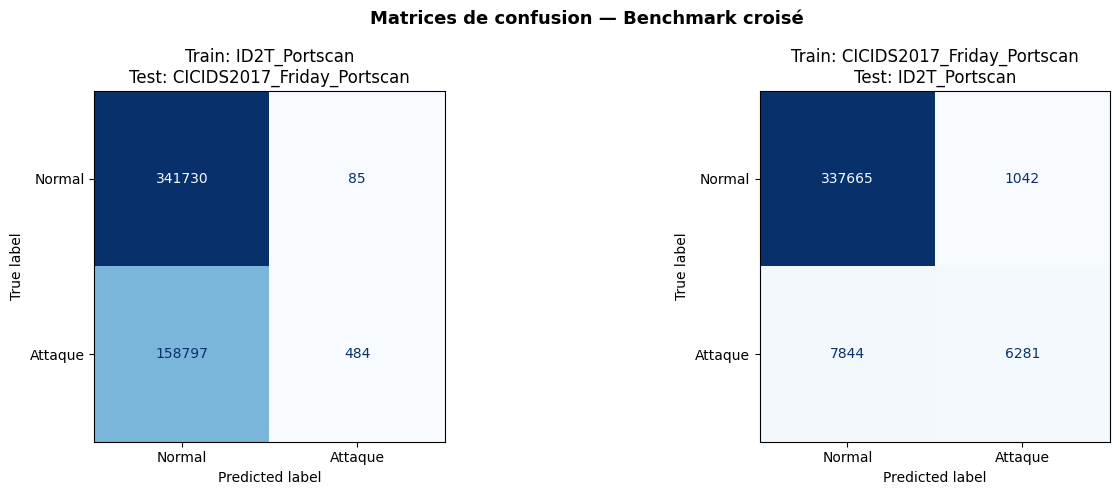
\includegraphics[width=\linewidth]{cm_cicids_id2t.png}
 \caption{Matrices de confusion -- benchmark croisé CICIDS2017 / ID2T.}
 \label{fig:cm_cicids}
\end{figure}
 
Le résultat le plus frappant concerne le sens \textbf{ID2T
$\rightarrow$ CICIDS2017}~: bien que la precision reste élevée
(85,06\,\%), le recall s'effondre à 0,30\,\%. Sur les 159\,281 flux
d'attaque présents dans le jeu de test CICIDS2017, seuls 484 sont
correctement détectés~; 158\,797 attaques réelles passent inaperçues.
Autrement dit, un modèle entraîné uniquement sur les PortScans générés
par ID2T est presque totalement incapable de détecter les mêmes
attaques lorsqu'elles proviennent d'une capture réelle.
 
Le sens inverse, \textbf{CICIDS2017 $\rightarrow$ ID2T}, donne des
résultats sensiblement meilleurs~: un recall de 44,47\,\% et un
F1-score de 58,57\,\%. Un modèle entraîné sur des attaques réelles
parvient à en détecter une partie significative parmi les attaques
générées par ID2T, sans toutefois s'en approcher parfaitement.
 
Cette forte asymétrie constitue une preuve empirique directe que les
attaques PortScan injectées par ID2T possèdent une signature
statistique sensiblement différente de celle des attaques PortScan
réelles de CICIDS2017. Le modèle entraîné sur le trafic généré apprend
des régularités propres à la méthode d'injection d'ID2T, qui ne se
retrouvent pas -- ou trop partiellement -- dans le trafic réel.
 
\subsection{Comparaison TON-IoT -- ID2T}
 
Le tableau~\ref{tab:results_toniot} présente les résultats du benchmark
croisé entre le dataset généré par ID2T à partir d'un fond bénin
TON-IoT et le dataset TON-IoT original.
 
\begin{table}[H]
\centering
\caption{Résultats du benchmark croisé TON-IoT -- ID2T (classe Attaque).}
\label{tab:results_toniot}
\small
\begin{tabular}{lccccc}
\toprule
\textbf{Train $\rightarrow$ Test} & \textbf{Precision} & \textbf{Recall} & \textbf{F1} & \textbf{FN} & \textbf{FP} \\
\midrule
ID2T $\rightarrow$ TON-IoT & 99,99\,\% & 78,29\,\% & 87,82\,\% & 16\,218 & 3 \\
TON-IoT $\rightarrow$ ID2T & 99,73\,\% & 100,00\,\% & 99,86\,\% & 0 & 20 \\
\bottomrule
\end{tabular}
\end{table}
 
\begin{figure}[H]
 \centering
 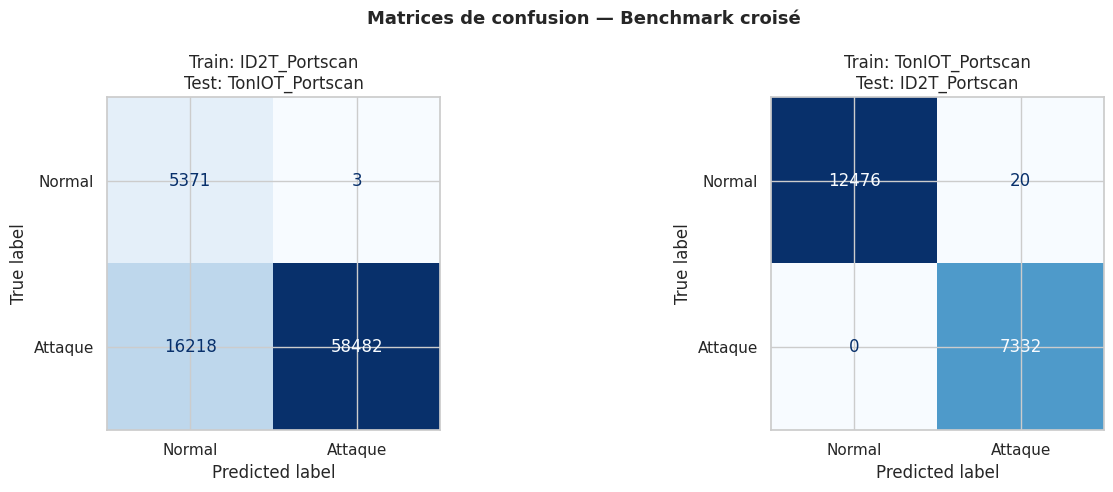
\includegraphics[width=\linewidth]{cm_toniot_id2t.png}
 \caption{Matrices de confusion -- benchmark croisé TON-IoT / ID2T.}
 \label{fig:cm_toniot}
\end{figure}
 
Ces résultats contrastent fortement avec ceux obtenus sur la paire
CICIDS2017 -- ID2T. Dans le sens \textbf{ID2T $\rightarrow$ TON-IoT},
le modèle atteint un recall de 78,29\,\%, très supérieur au 0,30\,\%
observé pour CICIDS2017. Dans le sens inverse, \textbf{TON-IoT
$\rightarrow$ ID2T}, le modèle obtient un score quasiment parfait
(recall de 100,00\,\%, aucun faux négatif).
 
Ce score parfait doit toutefois être interprété avec prudence. Comme
détaillé en section~\ref{sec:preprocessing}, le dataset
\texttt{ID2T\_Portscan} utilisé pour TON-IoT n'a pas pu être constitué
selon le pipeline standard ID2T~$\rightarrow$~NFStream~$\rightarrow$~labellisation,
en raison de la disparition du trafic bénin lors de la fusion~; il a
dû être reconstitué manuellement à partir d'un échantillon de flux
d'attaque et de flux bénins extraits séparément du même fichier
source. Il n'est pas exclu que cette reconstitution introduise une
proximité artificielle entre les flux d'attaque utilisés pour
l'entraînement (sur TON-IoT) et ceux utilisés pour le test (échantillon
tiré de la même source), ce qui pourrait expliquer, au moins en partie,
un score aussi élevé. En l'absence de vérification approfondie d'un
éventuel chevauchement entre les flux d'entraînement et de test, ce
résultat doit être considéré comme une limite méthodologique de cette
comparaison plutôt que comme une preuve définitive de généralisation
parfaite.
 
L'asymétrie modérée observée dans le sens \textbf{ID2T
$\rightarrow$ TON-IoT} (recall de 78,29\,\%, 16\,218 attaques
manquées sur 74\,700) reste néanmoins un résultat plus robuste, car il
n'est pas affecté par la reconstitution mentionnée ci-dessus. Il
suggère que les attaques générées par ID2T à partir d'un fond IoT
capturent une partie substantielle, mais non totale, des
propriétés statistiques des attaques PortScan réelles de TON-IoT,
un comportement nettement meilleur que celui observé sur CICIDS2017.
 
\section{Analyse qualitative par réduction de dimension}
\label{sec:qualitative_analysis}
 
Afin de mieux comprendre l'origine de ces asymétries, les flux des
deux paires de datasets ont été projetés dans un espace de dimension
réduite, à l'aide de deux méthodes complémentaires~: t-SNE, qui
préserve les structures locales de voisinage, et l'analyse en
composantes principales (PCA), qui préserve les directions de plus
grande variance globale.
 
\subsection{Comparaison CICIDS2017 -- ID2T}
 
\paragraph{Trafic normal.} La projection PCA du trafic normal
(figure~\ref{fig:pca_normal}) montre un chevauchement marqué entre les
échantillons originaux (CICIDS2017) et générés (ID2T). Les deux
nuages de points occupent globalement la même région de l'espace des
deux premières composantes principales, avec une large zone de
recouvrement dense. Ce résultat est cohérent avec le principe de
fonctionnement d'ID2T, le trafic bénin en sortie de l'outil
correspond au trafic bénin source, laissé inchangé par le processus
d'injection.
 
\begin{figure}[H]
 \centering
 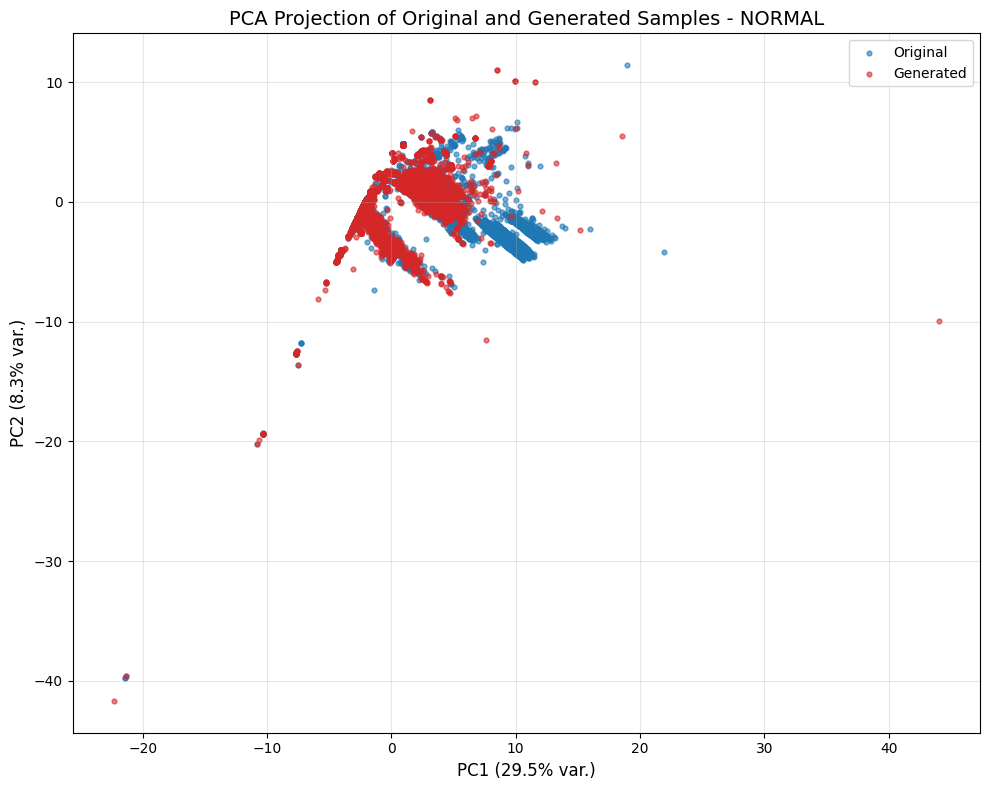
\includegraphics[width=0.85\linewidth]{pca_normal_cicids.png}
 \caption{Projection PCA du trafic normal -- original vs. généré (CICIDS2017 / ID2T).}
 \label{fig:pca_normal}
\end{figure}
 
\paragraph{Trafic d'attaque.} La projection PCA du trafic d'attaque
(figure~\ref{fig:pca_attack}) dresse un constat très différent~: les
échantillons originaux et générés forment deux nuages nettement
séparés dans l'espace des composantes principales, avec un
recouvrement nettement plus limité que pour le trafic normal. Cette
séparation visuelle confirme, au niveau de la structure globale des
données, ce que révélait déjà le recall quasi nul obtenu en
entraînement croisé. Les attaques générées par ID2T occupent une
région distincte de l'espace des features par rapport aux attaques
réelles de CICIDS2017.
 
\begin{figure}[H]
 \centering
 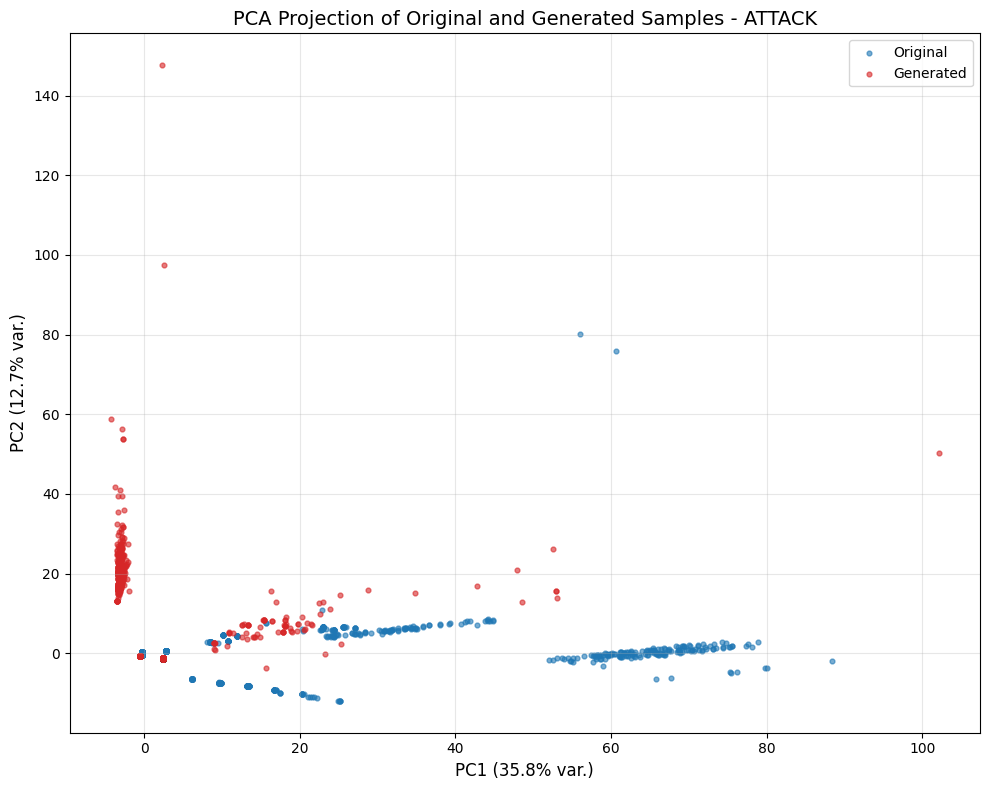
\includegraphics[width=0.85\linewidth]{pca_attack_cicids.png}
 \caption{Projection PCA du trafic d'attaque -- original vs. généré (CICIDS2017 / ID2T).}
 \label{fig:pca_attack}
\end{figure}
 
La visualisation t-SNE correspondante, bien que rendue moins lisible
par le faible nombre d'échantillons d'attaque après
sous-échantillonnage, ne contredit pas cette observation. Les points
correspondant aux attaques (réelles et générées) apparaissent
dispersés au sein de la masse de trafic normal plutôt que regroupés
en un cluster homogène commun, ce qui suggère l'absence d'un
chevauchement fort entre les deux distributions d'attaque au niveau
local.

\begin{figure}[H]
 \centering
 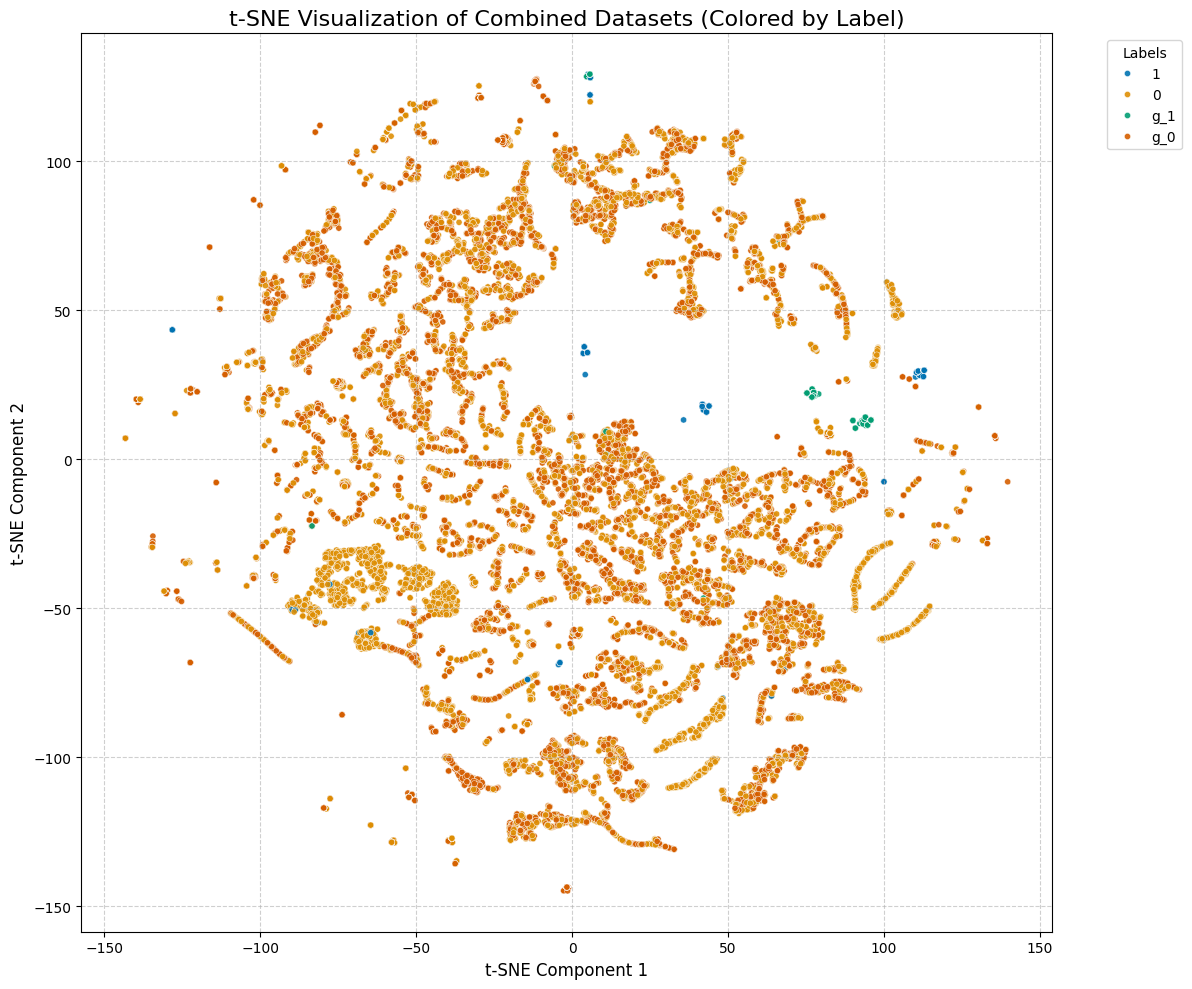
\includegraphics[width=0.85\linewidth]{tsne_cicids.png}
 \caption{Projection t-SNE du dataset combiné -- CICIDS2017 / ID2T.}
 \label{fig:tsne_cicids}
\end{figure}
 
\subsection{Comparaison TON-IoT -- ID2T}
 
\paragraph{Trafic normal.} La projection PCA du trafic normal pour la
paire TON-IoT -- ID2T (figure~\ref{fig:pca_normal_toniot}) montre un
comportement similaire à celui observé sur CICIDS2017. La majorité
des échantillons originaux et générés se superposent dans une zone
dense proche de l'origine, bien qu'un sous-ensemble d'échantillons
originaux et générés s'étende de façon plus dispersée le long de la
première composante principale, sans toutefois former deux groupes
distincts. Le recouvrement global reste donc satisfaisant, cohérent
avec le fait que le trafic bénin n'est jamais modifié par ID2T.
 
\begin{figure}[H]
 \centering
 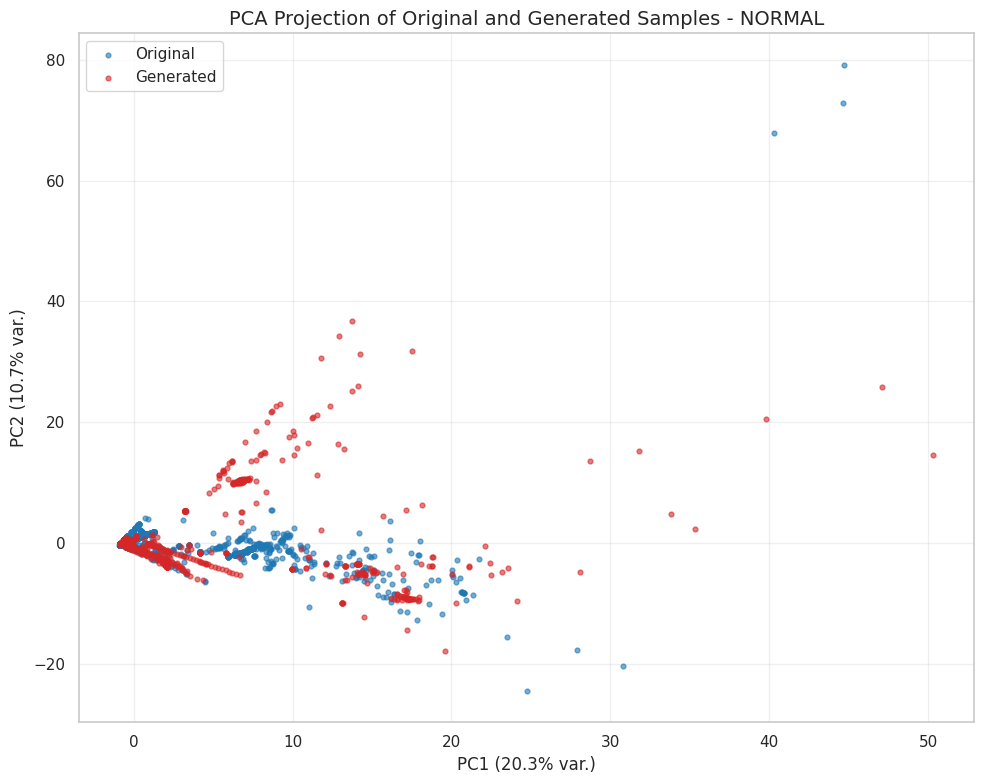
\includegraphics[width=0.85\linewidth]{pca_normal_toniot.png}
 \caption{Projection PCA du trafic normal -- original vs. généré (TON-IoT / ID2T).}
 \label{fig:pca_normal_toniot}
\end{figure}
 
\paragraph{Trafic d'attaque.} La projection PCA du trafic d'attaque
(figure~\ref{fig:pca_attack_toniot}) présente un résultat notable~:
les échantillons générés apparaissent concentrés en un point unique,
quasiment sans dispersion, tandis que les échantillons originaux
TON-IoT sont largement dispersés sur l'ensemble du plan des composantes
principales. Cette absence de variance dans les échantillons générés
est cohérente avec la reconstitution manuelle du dataset ID2T pour
TON-IoT décrite en section~\ref{sec:preprocessing}~: les flux
d'attaque disponibles pour cette paire proviennent d'un échantillonnage
restreint à partir d'un fichier unique, ce qui limite mécaniquement
leur diversité statistique et rend leur comparaison avec la PCA du
trafic d'attaque de CICIDS2017 (où les échantillons générés étaient
nettement plus dispersés) délicate.
 
\begin{figure}[H]
 \centering
 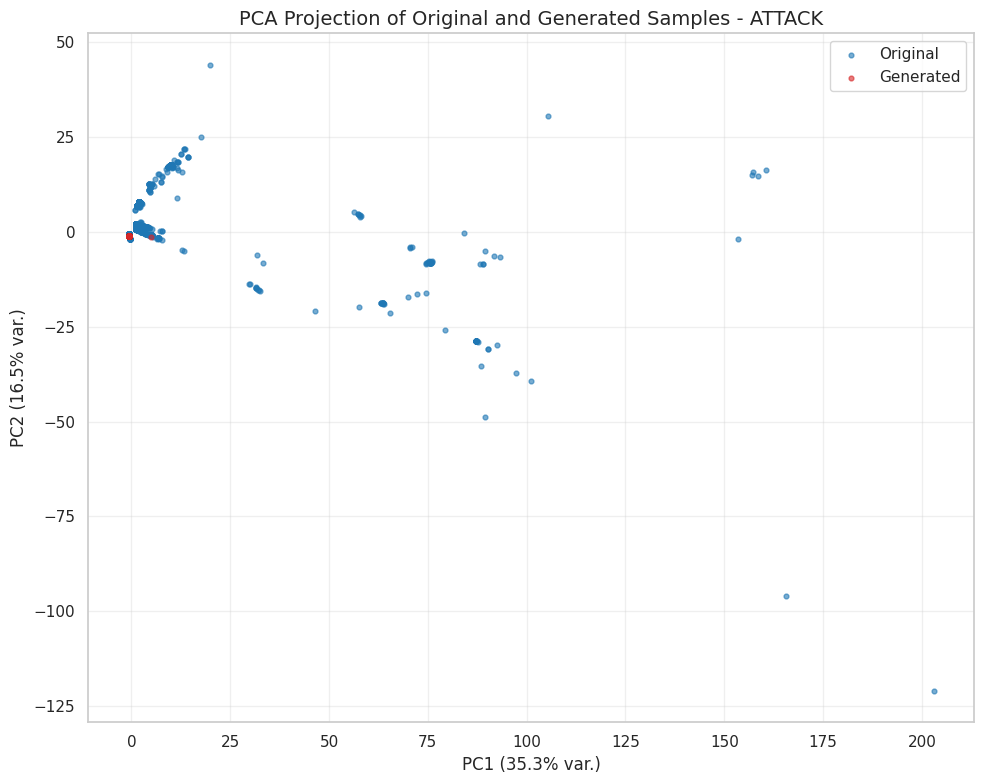
\includegraphics[width=0.85\linewidth]{pca_attack_toniot.png}
 \caption{Projection PCA du trafic d'attaque -- original vs. généré (TON-IoT / ID2T).}
 \label{fig:pca_attack_toniot}
\end{figure}
 
La visualisation t-SNE combinée (figure~\ref{fig:tsne_toniot}) permet
une lecture complémentaire~: les points générés (attaque et normal)
forment plusieurs petits amas compacts, dispersés à l'intérieur et en
périphérie de la structure formée par les points originaux, sans
recouper précisément les régions denses de trafic d'attaque réel
(orange). Ce comportement, plus favorable que celui observé sur
CICIDS2017 où les points générés étaient presque invisibles, doit
néanmoins être interprété prudemment au vu des réserves méthodologiques
énoncées précédemment.
 
\begin{figure}[H]
 \centering
 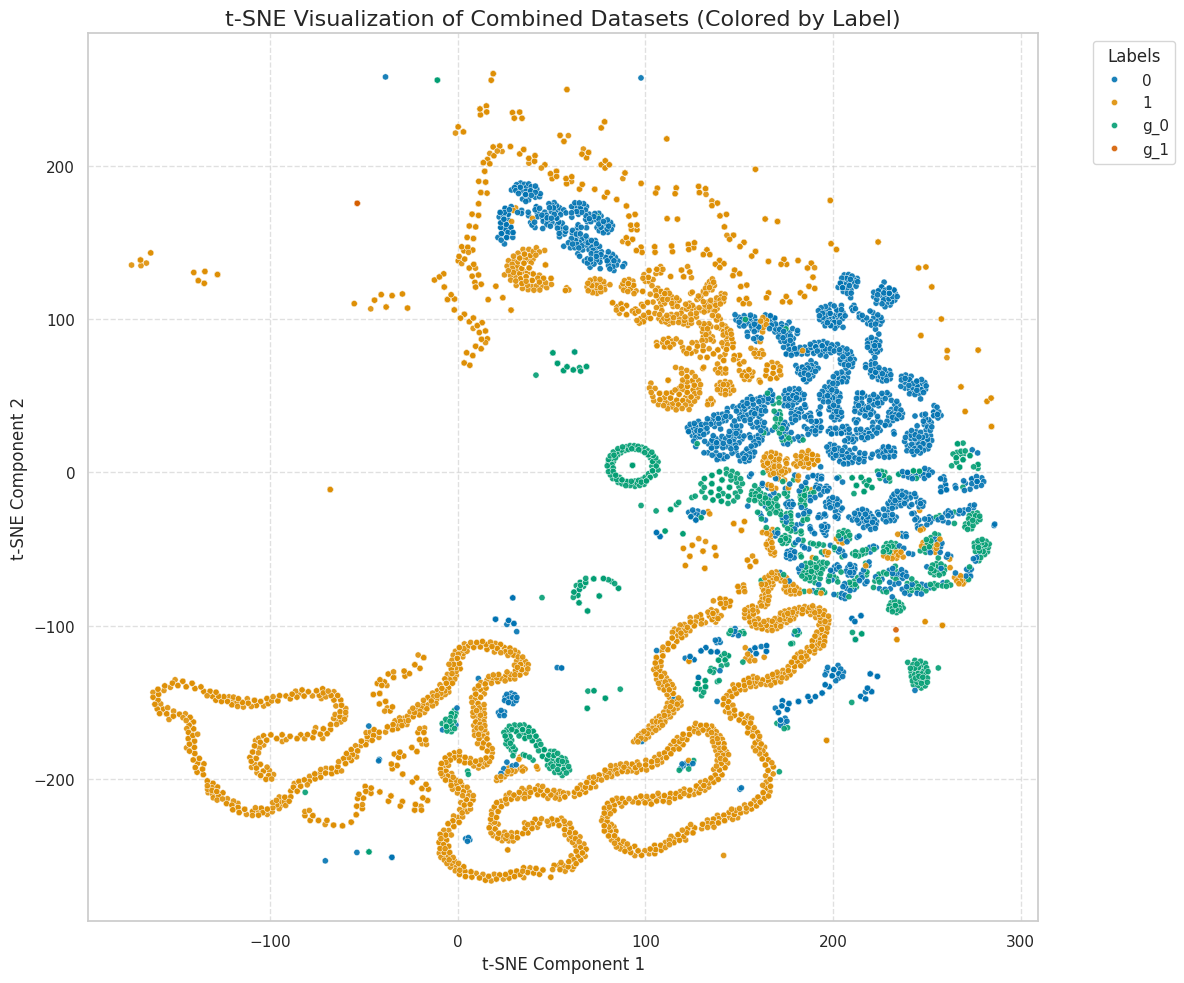
\includegraphics[width=0.85\linewidth]{tsne_toniot.png}
 \caption{Projection t-SNE du dataset combiné -- TON-IoT / ID2T.}
 \label{fig:tsne_toniot}
\end{figure}
 
\section{Synthèse des résultats}
 
L'ensemble des expériences menées dans ce chapitre converge vers un
constat en deux volets. D'une part, \textbf{le trafic bénin} généré par
ID2T reproduit fidèlement les propriétés statistiques du trafic bénin
source dans tous les cas testés, ce qui est cohérent avec le fait que
ce trafic n'est jamais modifié par l'outil.
 
D'autre part, \textbf{le trafic d'attaque} généré présente un réalisme
très variable selon le contexte réseau source~: la généralisation
cross-dataset est quasiment nulle sur un fond de réseau classique
(CICIDS2017), mais sensiblement meilleure sur un fond de réseau IoT
(TON-IoT), sous réserve des limites méthodologiques liées à la
reconstitution manuelle du dataset discutées en
section~\ref{sec:preprocessing}.
 
Ces résultats suggèrent que la qualité du trafic d'attaque produit par
ID2T \textbf{dépend du contexte réseau source} plutôt que d'être une
propriété constante de l'outil. L'interprétation de cette dépendance
et ses implications sont discutées au chapitre suivant.
 
 
 
 
 
% --------------------------------------------------------
\chapter{Discussion}
\label{chap:discussion}
% --------------------------------------------------------
 
\section{Interprétation des résultats}
 
Comme synthétisé en section~\ref{chap:mlp}, les expériences de ce
stage montrent que le réalisme d'ID2T n'est pas uniforme~: fiable pour
le trafic bénin, mais très variable pour le trafic d'attaque selon le
contexte réseau. Plutôt que de reprendre les métriques détaillées au
chapitre~\ref{chap:mlp}, cette section s'attache à interpréter ce
constat et à le resituer dans la littérature.
 
L'écart observé entre les deux paires de datasets testées soulève une
question centrale~: pourquoi le PortScan injecté par ID2T généralise-t-il
mieux sur un fond IoT que sur un fond de réseau classique~? Une
hypothèse plausible tient à la complexité relative du trafic de fond.
Le trafic bénin CICIDS2017 est nettement plus divers en termes de
protocoles, de profils d'hôtes et de comportements applicatifs que
celui de TON-IoT, dont le testbed est plus restreint et plus homogène.
Un trafic de fond plus simple offre moins de différences, ce qui rend plus difficile pour le MLP de faire la distinction entre le trafic généré et le trafic réel, rendant mécaniquement la généralisation
plus facile sur TON-IoT que sur CICIDS2017. Cette hypothèse reste
toutefois spéculative et nécessiterait une analyse de features plus
fine pour être étayée.
 
Ce constat rejoint et prolonge un point soulevé dans l'état de l'art,
Garcia Cordero et al.~\cite{id2t2021} valident ID2T principalement sur
des réseaux informatiques conventionnels, sans évaluation systématique
sur des environnements IoT. Les résultats de ce stage montrent que
cette absence de validation n'est pas un simple manque formel, le
comportement de l'outil diffère réellement selon le type de réseau.
Ce résultat mériterait d'être confirmé sur d'autres paires de
datasets et d'autres types d'attaques avant de pouvoir être
considéré comme une propriété générale de l'outil.
 
\section{Limites du travail réalisé}
 
Plusieurs limites doivent être prises en compte dans l'interprétation
de ces résultats.
 
\textbf{Un seul type d'attaque testé.} L'ensemble des expériences de
ce stage repose exclusivement sur l'attaque PortScan. Il est donc
impossible de généraliser les conclusions obtenues à d'autres types
d'attaques disponibles dans ID2T (DDoS, EternalBlue, etc.), dont le
comportement d'injection et le réalisme statistique pourraient différer
sensiblement.
 
\textbf{Bug non résolu sur le module Merger.} Le comportement anormal
observé sur TON-IoT (disparition du trafic bénin en sortie, cf.
section~\ref{chap:analyse}) n'a pas pu être diagnostiqué au niveau du
code ou des logs internes d'ID2T, faute de temps. La cause exacte de
ce bug reste donc une hypothèse (limite du module Merger face à
certaines structures de paquets), non confirmée formellement.
 
\textbf{Reconstitution manuelle du dataset TON-IoT~$\rightarrow$~ID2T.}
Comme discuté en section~\ref{sec:preprocessing}, l'impossibilité
d'extraire un dataset ID2T complet et natif sur TON-IoT a nécessité
une reconstitution manuelle du trafic bénin et d'un échantillon de
trafic d'attaque. Cette solution de contournement a permis de mener
les expériences malgré le bug rencontré, mais elle fragilise
l'interprétation du résultat obtenu dans le sens
TON-IoT~$\rightarrow$~ID2T, dont le score quasi parfait pourrait
partiellement refléter une similarité artificielle entre les jeux
d'entraînement et de test plutôt qu'une réelle qualité de génération.
 
\textbf{Absence de réplication à plus grande échelle.} Les expériences
ont été menées sur un couple de fichiers PCAP par type de réseau. Les
conclusions tirées, notamment sur la différence de comportement entre
réseau classique et réseau IoT, gagneraient à être confirmées sur un
plus grand nombre de captures sources, afin d'écarter la possibilité
que les résultats observés soient spécifiques aux fichiers utilisés
plutôt que représentatifs d'un comportement général de l'outil.
 
\textbf{Portée limitée du modèle MLP utilisé.} Le choix d'un MLP comme
unique modèle de classification, motivé par sa simplicité et sa
reproductibilité (cf. section~\ref{sec:features_mlp}), ne permet pas
de savoir si les constats faits ici, notamment la faible
généralisation sur CICIDS2017, se retrouveraient avec d'autres
architectures (CNN, LSTM) potentiellement plus ou moins sensibles aux
différences statistiques fines entre trafic généré et trafic réel.
Faute de temps, plusieurs approfondissements n'ont pas pu être menés,
une comparaison systématique de plusieurs architectures de
classification sur les mêmes datasets, une recherche d'hyperparamètres
plus poussée que la configuration unique retenue pour le MLP, ainsi
qu'une validation croisée (\textit{k-fold}) permettant d'estimer la
variance des résultats obtenus plutôt qu'un unique split
entraînement/test par expérience. Cela aurait montré si les écarts viennent du trafic d'ID2T ou des choix de modélisation.
 
 
 
 
 
% --------------------------------------------------------
\chapter{Conclusion}
\label{chap:conclusion}
% --------------------------------------------------------
 
\section{Bilan scientifique}
 
Ce stage avait pour objectif de mener une analyse approfondie de
l'outil ID2T, en examinant les features exploitées pour générer le
trafic d'attaque, son adaptabilité à différents types de réseaux, et
la cohérence des attaques injectées selon les protocoles présents dans
le trafic bénin source.
 
L'analyse structurelle (chapitre~\ref{chap:analyse}) a mis en lumière
le fonctionnement déterministe et modulaire d'ID2T, ainsi qu'un bug
silencieux du module Merger entraînant la perte du trafic bénin sur
certaines captures. L'évaluation cross-dataset par MLP
(chapitre~\ref{chap:mlp}) a ensuite permis de mesurer concrètement
le réalisme du trafic généré, révélant une forte dépendance au
contexte réseau source~: le trafic bénin est fidèlement reproduit dans
tous les cas, tandis que le trafic d'attaque ne généralise que
partiellement, avec des performances très contrastées entre réseau
classique et réseau IoT (cf. chapitre~\ref{chap:discussion} pour
l'interprétation de cet écart).
 
Au final, ces travaux confirment qu'ID2T reste un outil utile pour la
génération de datasets IDS, à condition que la fiabilité de ses
attaques synthétiques soit vérifiée empiriquement pour chaque contexte
d'utilisation plutôt que présumée acquise.
 
\section{Perspectives}
 
Plusieurs axes de poursuite se dégagent directement des limites
identifiées au chapitre~\ref{chap:discussion}.
 
\textbf{Diagnostiquer et corriger le bug du module Merger.} L'origine
exacte de la disparition du trafic bénin sur TON-IoT reste à identifier
avec précision. Une inspection du code source du Merger, associée à des
tests unitaires sur des captures TON-IoT réduites, permettrait de
localiser la cause du problème et, potentiellement, de proposer un
correctif à soumettre aux mainteneurs du projet.
 
\textbf{Étendre l'évaluation à d'autres types d'attaques.} Seule
l'attaque PortScan a été testée dans ce stage. Reproduire le protocole
d'évaluation cross-dataset sur d'autres attaques disponibles dans
ID2T (DDoS, EternalBlue, etc.) permettrait de déterminer si l'écart de
réalisme observé entre CICIDS2017 et TON-IoT se généralise, ou s'il est
spécifique au PortScan.
 
\textbf{Refaire la comparaison TON-IoT sans reconstitution manuelle.}
Une fois le bug du Merger résolu, il serait possible de régénérer un
dataset ID2T$\rightarrow$TON-IoT complet et natif, permettant de
recalculer le sens TON-IoT$\rightarrow$ID2T sans le biais potentiel
introduit par la reconstitution manuelle utilisée dans ce stage, et de
confirmer, ou d'infirmer, le résultat obtenu.
 
\textbf{Approfondir le volet apprentissage automatique.} Comme évoqué
en section~\ref{chap:discussion}, comparer plusieurs architectures de
classification, mener une recherche d'hyperparamètres plus systématique
et recourir à une validation croisée permettrait de consolider la
robustesse statistique des résultats présentés dans ce rapport.
 
\textbf{Poursuivre l'amélioration d'ID2T pour les datasets mixtes.}
Comme indiqué en introduction, l'ajout de la prise en charge de
plusieurs fichiers \texttt{.pcap} en entrée d'ID2T, envisagé initialement
comme second axe de ce stage, n'a pas pu être abordé faute de temps.
Cette amélioration permettrait de générer des datasets combinant
plusieurs sources de trafic bénin, par exemple un mélange de réseau
classique et de réseau IoT, ouvrant la voie à des scénarios de test
plus proches de la diversité des réseaux réels.
 
\section{Bilan personnel}
 
Ce stage a constitué une première expérience concrète du travail de
recherche, avec ses apports aussi bien techniques que méthodologiques.
 
Sur le plan technique, il m'a permis d'approfondir mes connaissances en
apprentissage automatique appliqué à la cybersécurité, de manipuler des
outils spécialisés dans l'analyse de trafic réseau (ID2T, NFStream), et
de développer des scripts de traitement de données pour résoudre des
problèmes concrets de préprocessing rencontrés en cours de route,
notamment l'hétérogénéité des formats entre outils de génération de
flux réseau.
 
Sur le plan méthodologique, ce stage m'a surtout confronté à une
dimension du travail de recherche que je ne maîtrisais pas encore.
La rigueur nécessaire face à l'incertitude. Le rythme du travail de
recherche diffère sensiblement de celui d'un projet académique classique
au résultat attendu. Un résultat inattendu, comme le bug rencontré sur
TON-IoT ou l'asymétrie marquée des scores cross-dataset, n'est pas un
échec mais une donnée à part entière, qu'il faut savoir documenter,
questionner et replacer dans son contexte plutôt que d'en tirer des
conclusions hâtives. Cette exigence de prudence dans l'interprétation
des résultats, en particulier lorsqu'un score semble \textit{trop} bon
pour être pleinement fiable, constitue à mon sens l'un des apprentissages
les plus utiles de cette introduction au monde de la recherche.
 
 
% ============================================================
%  BIBLIOGRAPHIE
% ============================================================
\printbibliography[heading=bibintoc, title={Références bibliographiques}]
 
 
% ============================================================
\end{document}
% ============================================================